\chapter{解题报告}
\begin{center}
\begin{longtable}{l c c c c c }

Date & Problem ID & Title & Difficulty & Type & Person   \\ 
\hline
2022-12-20 & CF1763E & Node Pairs & 2200 & 图论、最优性构造 & zmy  \\
2023-12-11 & CF1904E & Tree Queries & 2500 & 图论, 树论 & shaosy \\
2023-12-14 & CF1904F & Beautiful Tree & 2800 & 图论, 树论 & shaosy \\
2023-12-14 & CF1903F & Babysitting & 2500 & 图论 & shaosy \\
2023-12-22 & CF1913E & Matrix Problem & 2400 & 图论 & shaosy \\
2023-12-22 & CF1905E & One-X & 2400 & 分治, 线段树 & shaosy \\
2023-12-24 & CF1909E & Multiple Lamps & 2400 & 暴力, 构造 & shaosy \\
2023-12-25 & CF1909F & Small Permutation Problem (Easy Version) & F1 2200, F2 2500 & DP, 计数 & pufanyi \\
2023-12-25 & CF1917E & Construct Matrix & 2500 & 存在性构造 & shaosy \\
2023-12-25 & CF1917F & Construct Tree & 2500 & 背包, 构造 & shaosy \\
2023-12-28 & CF1854C & Expected Destruction & 2500 & DP, 概率 & shaosy \\
\hline

\label{tab:practice_index}
\end{longtable}
\end{center}
\section{Codeforces}

\ptitle{[CF1763E] Node Pairs}{zmy}
\prob 要求构造一个有向图,恰好有 $p (1 \leq p \leq 2 \cdot 10^5)$ 个点对互相可达。在这个前提下,要求使用的顶点数尽可能少。顶点数相同时,要求单向可达的点对尽可能多
\sol 每个有向图都可以被缩点成一个 DAG,对于每个强连通分量内部肯定是两两可达的,且夸强连通分量的点对一定不是双向可达的。因此我们可以想到用 DP 来计算需要的最小顶点数。再次之上,为了使得单向可达的点对尽可能多,我们的 DAG 一定是一条链的形状,因此我们可以同时 dp 单向可达的点对个数。

\ptitle{[CF1904E] Tree Queries}{shaosy}
\prob 给定一棵树, 多组询问. 每组询问指定一个询问点和一些删除点, 问将删除点删除后树中询问点可达的最远距离为多少
\sol 离线处理. 首先, 询问某一点在书中可达最远距离等价于将该点视为树的根并询问树的深度. 考虑如何换根时更新树的深度. 考虑dfs序. 通过维护每个点的in和out时刻, 配合线段树, 可以用换根dp类似的思想来动态维护每个点当前的深度. 根通过边u-v从u换到v等价于, 给v的子树深度区间减1, 给其他节点深度加1. 然后讨论删除点. 删除点如果在原树中不是新的根节点(x) 的父节点,则可以视作将删除点的子树的深度区间减去正无穷. 而如果是, 则可以视作将除了删除点与点x相连的子树之外所有点的深度区间减去正无穷. 在这种更新下, 当前树的深度就是所有点深度的最大值.

\ptitle{[CF1904F] Beautiful Tree}{shaosy}
\prob 给定一棵树和多组限制条件,要求给树上每一个点赋值使得其成为一个permutation并满足所有限制条件. 每组限制条件形如 u-v-x, 要求使得在路径u-v上的点中x的值最大/最小
\sol 考虑树链剖分+线段树优化建图. 这样, 每一段树上路径可以用不超过$\log{n}$个线段, 每个线段又不超过$\log{n}$个点表示. 建立两颗线段树, 分别表示区间最大的点/区间最小的虚拟点, 而后暴力连边. 暴力连边后跑一边拓扑排序即可. 若存在环,则说明不存在可行解. 线段树优化建图中需要注意为了避免出现自环, 对路径u-v向路径x连边/或其反边连边时, 需要特判x是否在该路径中. 如果在该路径中必须裂成u-x和x-v两段(不包括x)

\ptitle{[CF1903F] Babysitting}{shaosy}
\prob 给定一个图, 选一些点形成一个点覆盖. 要求选的点之间相邻的差最小的最大.
\sol 考虑二分答案后2-SAT. 假设二分的答案为dif. 答案形成点覆盖等价于对每一条边u, v, 必然选择u和v中的一个. 相邻的差至少为dif等价于选择点u, 则不可选择范围为[u - dif + 1, u + dif - 1]中的任意一个点. 这一性质满足2-sat, 可以在其上用线段树优化建图的trick将点数压缩到$O(n)$级别. 对线段树优化建图而言, 可以视作不选择u则必然不选择u * 2和u * 2 + 1

\ptitle{[CF1913E] Matrix Problem}{shaosy}
\prob 给定一个矩阵, 每个矩阵的元素为0或1. 要求修改尽可能少的元素, 使得每一行的和为a[i], 每一列的和为b[i]. $n \leq 50, m \leq 50$
\sol 注意到数据范围很小, 考虑网络流. 如果对矩阵里每个元素建点, 则无法表示同一个点对行和列的贡献. 考虑将矩阵里的每一个点用边来表示, 即, 将$s$ 与行连边,列与$t$连边,点$i-j$由边表示. 若该点本身为$0$, 则将其代价设为$1$, 表示若将该点选择(流进该点)需要付出一点代价, 反之则将其代价设为$0$. 跑最小费用最大流, 则可得出一个新图, 该新图含义为, 满足题目要求, 且与原图最相似(修改点数最少/尽可能使用原图的边)的构造. 该最小费用最大流的流量即为新图的点数, 费用即为原图中删除(修改)的点数. 则总代价即为 $c + (f - (sum - c))$, 其中$sum$ 为原图中的点数.

\ptitle{[CF1905E] One-X}{shaosy}
\prob 给定一颗线段树. 对于其叶子的所有子集, 求其LCA的和, 数据范围1e18. 具体的, build的定义为build(v,l,r), 令$m = (l+r)/2$(向下取整), 将v和2v与2v+1连边, 后递归调用build(2v,l,m)和build(2v+1,m+1,r)
\sol  考虑单个点的可能贡献. 假设该点的左子树区间长度为$l$, 右子树区间长度为$r$, 显然有点$x$的贡献为$x \times (2^l - 1) \times (2^r - 1)$. 考虑线段树的性质, 发现对相同层的$x$, 其$l$和$r$必然为$\lfloor{\frac{x}{2}}\rfloor$和$\lceil{\frac{x}{2}}\rceil$中的一个. 接下来考虑一个区间长度固定的子树答案. 这一部分可以由两个部分组成: 与$x$相关的($k$) 和 与$x$无关的($b$). 其形式必定如$k\times x + b$

考虑如何更新$k$.首先, $k$必然包括$(2^l-1) \times (2^r - 1)$, 这是由LCA为点$x$的集合数量. 接下来考虑两颗子树$l$和$r$. 首先, $l$和$r$的差至多为1, 假设$l$是较长者. 则$k_l$所能作出的贡献为$2 * v + 1$, 而$k_r$所能作出的贡献为$2 * v$. 于是, 将与$v$相关的部分纳入考虑, 无关部分交给$b$, 即可得出$k = 2k_l + 2k_r + (2^{l}-1) \times (2^{r} - 1)$, $b = b_l + b_r + k_l$. 本质不同的$k,b$对不超过$2\log{n}$个. 可以通过记忆化所搜得到答案.

\ptitle{[CF1909E] Multiple Lamps}{shaosy}
\prob 给定$1$到$n$组灯(一开始均为暗). 每个灯只能被按一次. 按第$i$个灯会切换所有的第$k \times i$个灯. 有$m$组限定条件, 形如$u, v$, 表示如果按灯$u$必定按灯$v$(顺序无要求, 因为每个灯最多按一次). 求是否存在一组构造使得最后总共亮的灯的个数小于等于$n / 5$.
\sol 首先, 考虑如果将所有的$i$都按一边. 在这种情况下, 只有所有的完全平方数的灯会亮. 在$n \geq 20$的情况下满足提议. 故我们仅需要考虑$n < 20$ 的情况.

在这种情况下, 最后亮的灯数必然小于等于$3$. 假设最后亮的灯中最小一个为第$i$个, 则显然, 该灯必然是被按下的(若$i$不是被按下的, 则存在另一个灯$j < i$且$j$为$i$的因数被按下, 与$i$是最小的亮的灯矛盾). 那么可以消除灯$i$的影响然后递归. 最后只需要检查按下的灯是否满足条件限制即可.

\ptitle{[CF1909F] Small Permutation Problem (Easy Version)}{pufanyi}
\prob 给你一个序列 $a$,求有多少个 permutation $p$ 使得对于任意 $i$,在 $p_1\sim p_i$ 小于等于 $i$ 的个数。 F1和F2的唯一区别是, F2存在$a_i = -1$, 表示对$a_i$没有限制
\sol Hard 还不会 qaq。首先考虑到是分三种情况讨论,$a_i-a_{i-1}$ 为 $0, 1, 2$。

第一个结论是我们定义一个自由度 $k_i$,表示 $p_1\sim p_i$ 中有多少个是可以大于 $i$ 的。其实我们发现 $k_i=i-a_i$,也就是说 $k_i$ 对于每个 $i$ 是固定的,不会根据 $1\sim i$ 中 $p$ 值的具体填法而造成改变。

第二个结论是一个可行的 $a$,必定满足 $a_i-a_{i-1}$ 为 $0$ 和为 $2$ 的数量相等。因为如果不相等的话,$a_n$ 加不到 $n$。

第三个结论是如果 $a_i-a_{i-1}=2$,那么 $1\sim i-1$ 中一定有一个 $i$,这个摸一下就行了。

然后我们令 $f_i$ 表示 $1\sim i$ 中,不考虑这 $k_i$ 个元素的答案。我们发现对于每个 $0$,事实上是增加了一个自由度,也就是 $p_i$ 可以填一个比 $i$ 大的数,而由于 $p_i$ 算在自由度中,所以我们不考虑他的贡献,于是 $f_i=f_{i-1}$。如果是 $2$,那必定是消耗了一个自由度,也就是说必须找到前面 $k_i$ 中的一个填成 $i$,所以 $f_i=f_{i-1}\times k$。

最后比较难办的是 $1$。我们考虑 $1$ 可能有两种情况:$1\sim i$ 中有 $i$ 并且 $p_i>i$ 和 $1\sim i$ 中没有 $i$ 并且 $p_i\le i$。但是需要注意的是根据第一个结论,不管哪种情况,自由度都只是加 $1$。因此我们其实不需要关注加的是哪一个,因为最后对自由度的贡献都是一样的。

如果 $1\sim i$ 中有 $i$ 并且 $p_i>i$,那么需要选择前面 $k_i$ 个中的一个作为 $i$,因此贡献为 $f_{i-1}\times k_i$。

如果 $1\sim i$ 中没有 $i$,那么 $p_i\le i$,$p_i$ 可以选择所有小于等于 $i$,并且前面没选过的数字。我当时在写的时候是直接考了一个新的变量统计了一下。写完发现好像就是 $i-a_i-1$。于是贡献就是 $f_{i-1}\times (i - a_i - 1)$。

于是式子是 $f_i=f_{i-1}\times (k_i+i-a_i-1)$。

\sol Fanyi的F1想麻烦了qaq. 其实有个简单点的做法(根据题解). 

首先, 题目要求构造一个permutation, 而构造一个permutation可以视为在一个$n \times n$的矩阵中填数字, 在点$(i,j)$中填数字即意味着令$p_i = j$. 那么, permutations的限制条件即等价于该矩阵中每一行每一列必然只有一个数字. 接下来考虑第二个限制条件, 对$i$要求小于等于$i$的数字个数等于$a_i$, 这就等价于在从$(1,1)$到$(i,i)$的子矩阵中, 有且仅有$a_i$个点. 在$F_1$中, 由于$a_i \not = -1$, 令$a_0 = 0$, 有$dif = a_i - a_{i-1}$, 则该限制条件可以转化为在L形(即$x = i, y \leq i$或$y = i, x \leq i$)中填写$dif(0,1,2)$个数字, 并且保证每行只有一个/每一列只有一个. 不难发现, 在维护当前已经填写了$k$个数字的情况下, 这一方法数对每一个L形都是独立的. 若$dif = 0$, 则只有一种; 若$dif = 1$, 则有$2 * (i - 1 - k) + 1$种; 若$dif = 2$, 则有$(i - 1 - k)^2$种方案.

F2也是用类似的方法解决. 和F1相比, 唯一的区别是存在一些$a_i$没有限制. 那么我们可以忽略这些$a_i$, 因为尾一定是$n$. 那么, 问题就转换为一个更大的L型(宽度不为1), 要求填充了. 对此, 我们可以枚举有多少个点在上部, 多少个点在下部. 

假设之前我们已经填充了$x_0 \times x_0$的矩阵, 有$y_0$个点; 我们现在要填充$x_1 \times x_1$的矩阵, 有$y_1$个点. 枚举有$k$个点放在上部(即这$k$个点存放在$p_{x_1} \sim p_{x_2}$中间, 且值小于等于$x_1$), 那么这$k$个点的贡献即为$\binom{x_1 - x_0}{k} \times \text{P}(x_0 - y_0, k)$. 剩余的$y_1 - y_0 - k$个点的贡献类似, 为$\binom{x_1 - x_0}{y_1 - y_0 - k} \times \text{P}(x_1 - y_0 - k, y_1 - y_0 - k)$

\ptitle{[CF1917E] Construct Matrix}{shaosy}
\prob 构造一个$0/1$矩阵, 长和宽均为$n$, 其中$n$为偶数, 使得总共有$k$个1, 并且每一行的$XOR$和一样, 每一列的$XOR$和一样.
\sol 显然, 因为$n$为偶数, 如果$k$为奇数则一定无解. 在$k$为偶数的情况下, 分类讨论. 发现$n\times n$的矩阵能够被$2 \times 2$的矩阵覆盖, 而$2 \times 2$的矩阵如果全部为$0/1$则不会影响每一行/列的$XOR$和. 所以, 如果$k \equiv 0 \pmod{4}$, 则显然可以构造一组解. 接下来考虑$k \equiv 2 \pmod{4}$的情况.

通过手玩可以发现, 在$k = 2$或$k = n^2 - 2$的情况下, 除非$n=2$, 则一定无解. 考虑其他情况. 此时, 一定有$k \geq 6$. 考虑$k = 6$和$k = n^2 - 6$情况下的特解, 可以发现两个如下的$4 \times 4$的矩阵能够满足要求:
$$
\begin{pmatrix}
1 & 1 & 0 & 0 \\
1 & 0 & 1 & 0 \\
0 & 1 & 1 & 0 \\
0 & 0 & 0 & 0 \\
\end{pmatrix}
\quad
\begin{pmatrix}
0 & 0 & 1 & 1 \\
0 & 1 & 0 & 1 \\
1 & 0 & 0 & 1 \\
1 & 1 & 1 & 1 \\
\end{pmatrix}
$$

那么, 我们只需要特判是否为$k = n^2-6$, 随后问题就与$k \equiv 0 \pmod{4}$等价了.

\ptitle{[CF1917F] Construct Tree}{shaosy}
\prob 给定一组边$l$(有边权), 构造一棵树使得树的直径为$d$
\sol 首先, 对$l$由大到小排序. 显然, 若有$l_0 + l_1 > d$则无解. 若背包得出不存在一组子集和为$d$, 也显然无解. 考虑背包存在子集$S$和为$d$的无解情况. 此时, 必然因为存在一条更长的直径大于$d$. 假设已经构造出这棵树, 则最优构造情况下, 所有非直径边必然连与同一个点, 而该点最优情况下显然尽可能于直径中间. 那么, 假设该点到直径两端距离为$x, y$, 若存在$l \not \in S$且$l > \min(x,y)$时, 无解.

为了简化考虑, 可以分类讨论$l_0$是否在$S$中间. 若$l_0$在$S$中, 则显然有解, 因为可以将$l_0$置于直径的一端, 后将所有非$S$边均与$l_0$非叶子的点相连. 在$l_0 + l_1 \leq d$的情况下, 始终符合题意.

若$l_0 \not \in S$, 我们可以仅考虑$l_0$是否满足$l_0 > \min(x,y)$. 首先, 因为$x + y = d$, 若$l_0 > \frac{1}{2} d$, 则该等式始终无法满足. 我们可以假设$l_0 \leq \frac{1}{2}d$. 接下来可以做一个背包, 令$dp[i][j]$为是否能够构造一条链, 使得链可以分为长度为$i$和长度为$j$的两部分. 对于每个$l[i]$, 分类讨论他应该在前半部分还是后半部分 dp[j + l[i]] |= dp[j], dp[j] |= (dp[j] << l[i]) 即可. 背包结束后, 仅需判断是否存在半边为$l_0$到$k - l_0$之间的任意解即可.

\ptitle{[CF1854C] Expected Destruction}{shaosy}
\prob 给定一个大小为$n$的set, 每次选择一个元素加一, 若加一后该元素$> m$或该元素与另一个元素相同, 则删除该元素. 求该set清空所需要的数学期望
\sol 假设在该set的末尾有一个位置在$m + 1$ 的不动点. 不难发现, 每次删除点都可以视作删除一对$i,j$中的一个点. 由于点之间没有区别, 我们可以认为每次删除的都是较大的$j$. 例如, 如果点$x$一直加到$y$, 我们可以视作原本的$y$被消除了, 而原本的$x$不过是位置变成了现在的$y$. 于是, 对每一个点$i$, 我们都可以假设点$i+1$永不消失. 那么, 每个相邻点对的贡献都是独立问题, 且仅和这两个点的初始位置相关.

那么, 可以定义$dp_{i,j}$为初始位置在$i$和初始位置在$j$的点相遇(消除一个)时, $i$点所走过的路程. 于是, 即有$dp_{i,j} = \frac{1}{2}(dp_{i+1, j} + 1 + dp_{i, j+1})$. 由于任意两个相邻点之间的贡献都是独立问题, 所以答案即为所有相邻点的贡献的和.

\ptitle{[CF1919F] Wine Factory}{shaosy}
\prob 有$n$个塔, 源点与每个塔有$a_i$的边, 汇点与每个塔有$b_i$的边, 塔$i$与$i+1$有权值为$c_i$的有向边, 每次更新一组$a_i, b_i, c_i$, 求最大流
\sol 由于数据范围过大, 不能直接最大流. 考虑最大流最小割定理, 最大流必然等同于最小割, 考虑如何去维护最小割.

假设: 对存在的最小割而言, 对每一个$i$, 必然割且仅割$a_i$和$b_i$中的一条边.

证明: 首先, 至少割一条边是显然的. 考虑若同时割去$a_i$和$b_i$时为何必有一条边多余. 首先, 在不考虑点$i$的情况下(即同时割去$a_i$和$b_i$), 结果也一定是一组割. 假设源点可以通过边$i-1 \to i$连接到点$i$, 则源点也一定可以通过该方法连接到点$i+1$. 那么,  我们可以发现, 在这种情况下, 边$a_i$没有必要割去. 假设源点不可以连接, 则可以发现, 在这种情况下, $a_i$和$b_i$只有一个需要割去即可. 

那么可以根据这个性质构建线段树. 发现如果需要合并两个相邻的点, 仅当点$i$为$b_i$而$i+1$为$a_i$时需要加上$c_i$的代价. 线段树上每个节点代表这个区间开始和结束点的选择为$a$还是$b$即可.
\section{AtCoder}

\ptitle{[AGC035C] Skolem XOR Tree}{pufanyi}

\prob 给 $n\ (n\le 10^5)$ 个白点 $n$ 个黑点,标号分别为 $1\sim n$。现在需要把这 $2n$ 个点连成一棵树,使得编号为 $i$ 的白点和黑点路径的 xor 和为 $i$。有可能无解。
\sol 如果 $n=2^k$,我们发现第 $n$ 个白点和黑点路径 xor 和的第 $k$ 位肯定是 $0$,那无解。

如果 $n$ 是奇数,我们考虑这样构造:

\begin{center}
    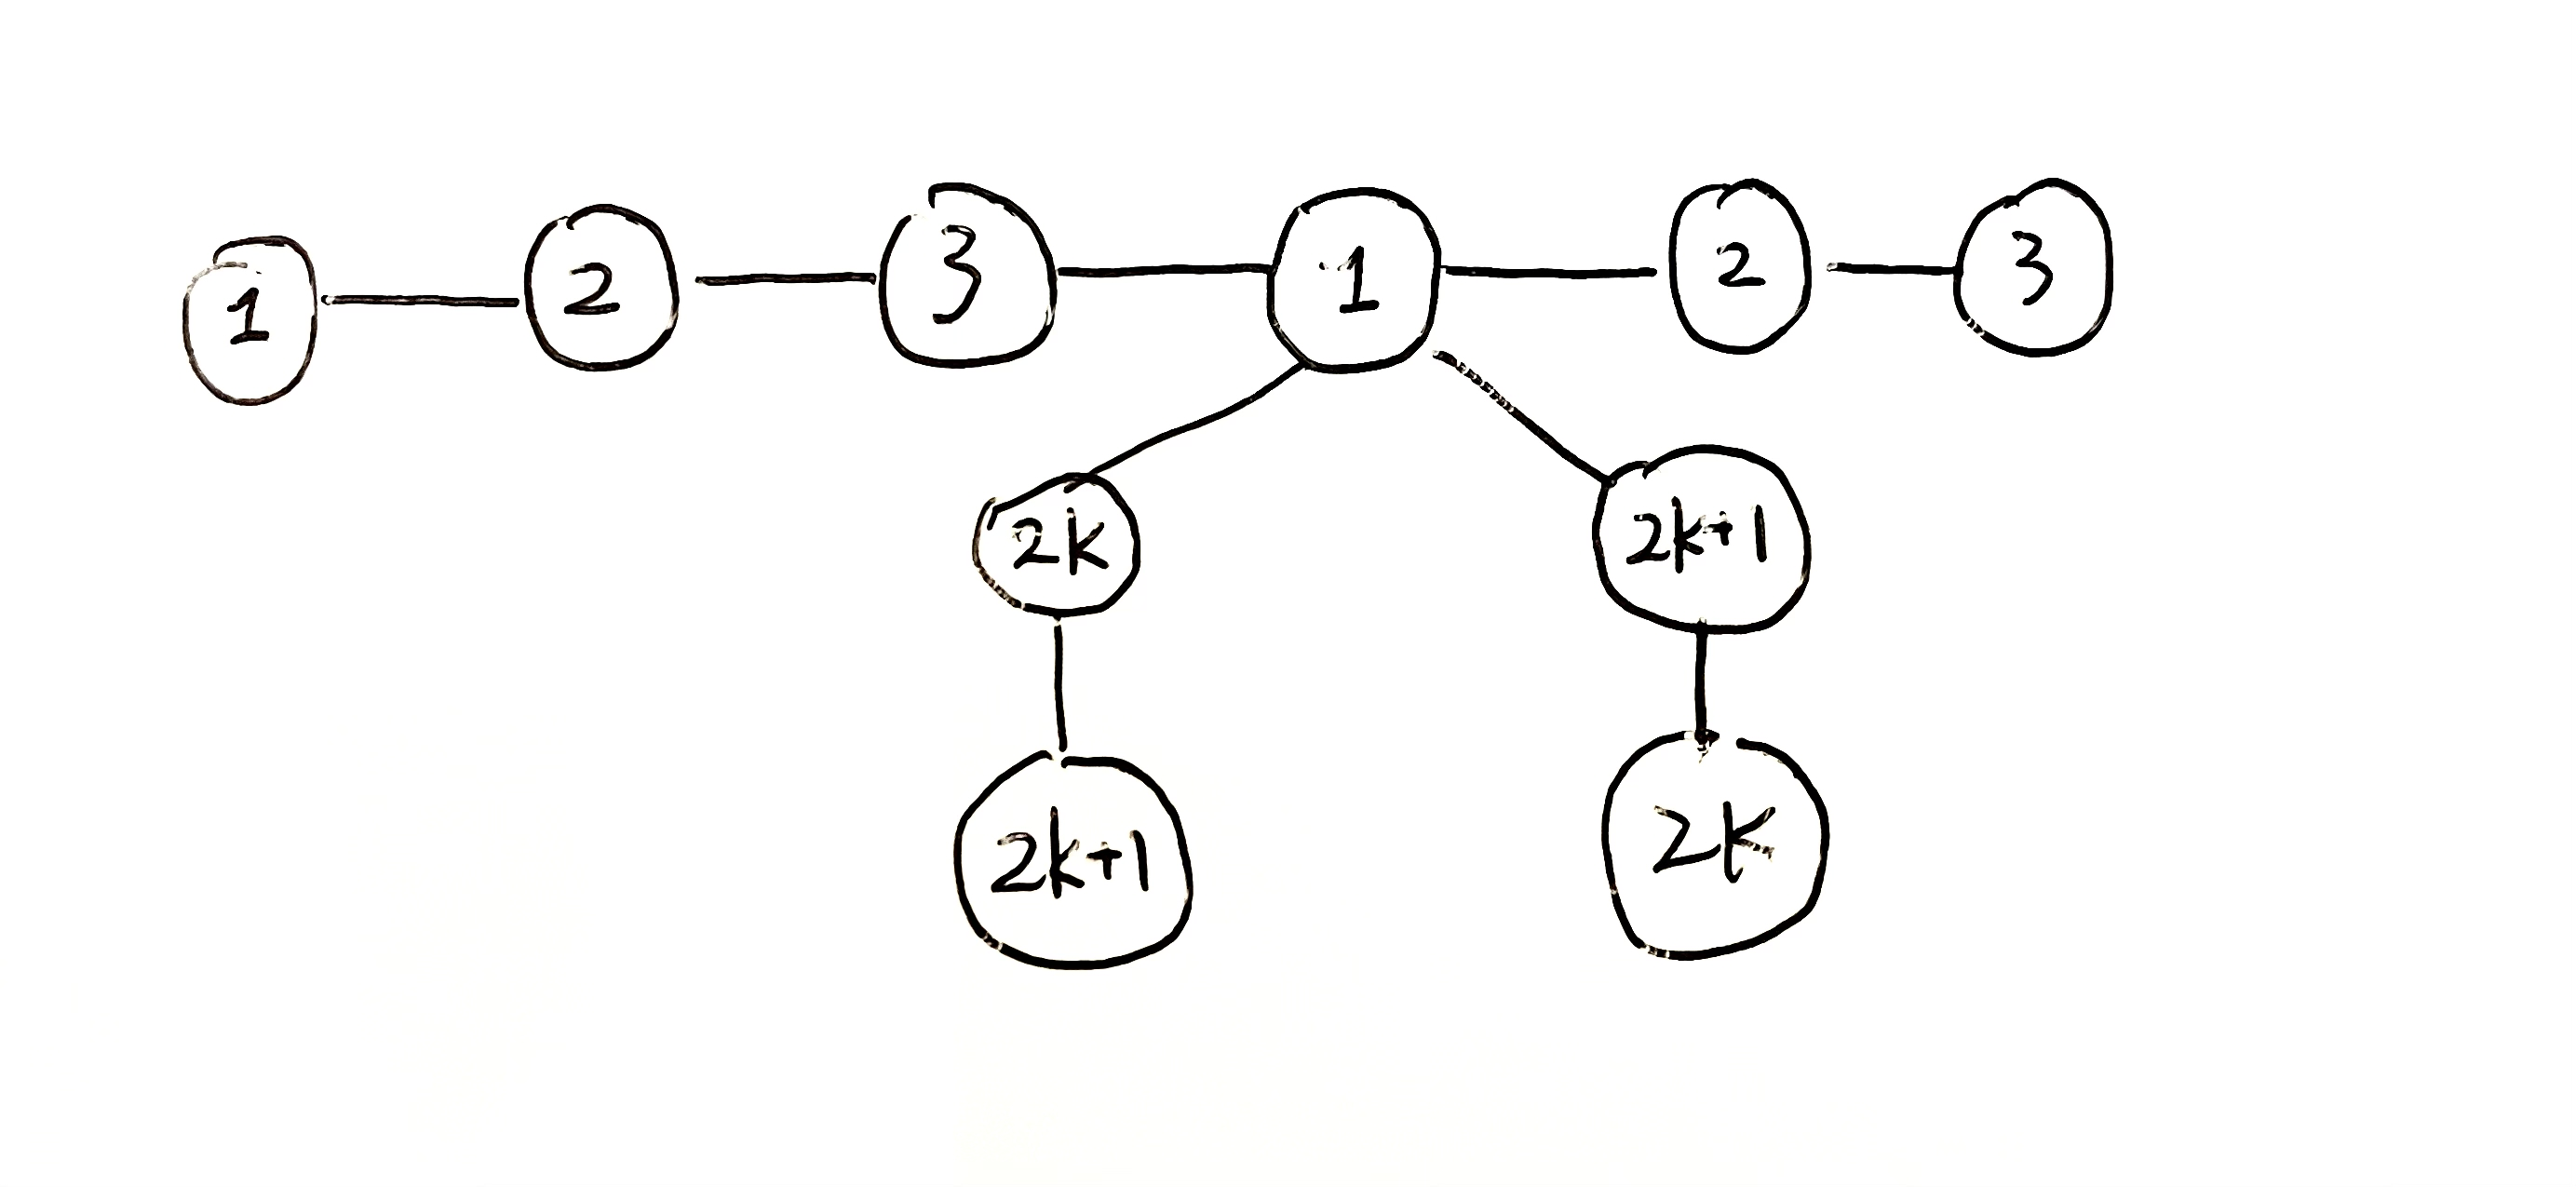
\includegraphics[width=0.7\textwidth]{solutions/img/agc035c/agc035c.jpg}
\end{center}

然后我们考虑 $n$ 是偶数的情况,我们考虑先构造出 $n-1$ 的答案,然后找到最大的 $m=2^k<n$,然后我们连接 $n\sim m\sim 1\sim (n-m+1)\sim n$ 即可。

关于 $n$ 是偶数的情况听了一下他的 tutorial,他大概是这样想的:因为 $1$ 连了 $2\sim n-1$ 的点,一个简单的思想是能不能找到 $n\sim a\sim 1\sim b\sim n$ 使得 $n\bigoplus a\bigoplus 1\bigoplus b\bigoplus n=n$,于是可以得到 $a\bigoplus b=n+1$,这时候想到 $m\bigoplus (n-m+1)=n+1$ 比较自然。

\ptitle{[AGC026F] Manju Game}{pufanyi}

\prob 有 $n$ 个箱子排成一列,第 $i$ 个箱子价值为 $a_i$。先手先随便选一个箱子并将其拿走。接着,两个人轮流操作,如果上一个人选的箱子为 $i$,那当前这个人只能选 $i-1$ 或者 $i+1$ 两个箱子中的其中一个。如果这两个箱子已经都被人拿走了或者不存在,那么这个人可以任意在这个序列中选择一个没被取过的箱子并且取走。如果两个人都是聪明的,他们都想得到箱子的价值和最大化,求最终先手和后手得到的价值。
\sol 假设所有奇数箱子的价值和为 $A$,偶数箱子的价值和为 $B$。

如果 $n$ 为偶数,摸一下不难发现答案为 $\left<\max\{A, B\}, \min\{A, B\}\right>$。

现在考虑 $n$ 为奇数的情况。我们分类讨论当前情况下先手选的是奇数箱子还是偶数箱子。偶数箱子比较好讨论,因为他把两边划分成了两段奇数箱子。这时候后手需要选一个方向进行取箱子。将这个方向的箱子取完后,我们发现留下了奇数个箱子,这时候当前的先手仍然是原来的先手,于是就变成了一个递归问题。

\begin{center}
    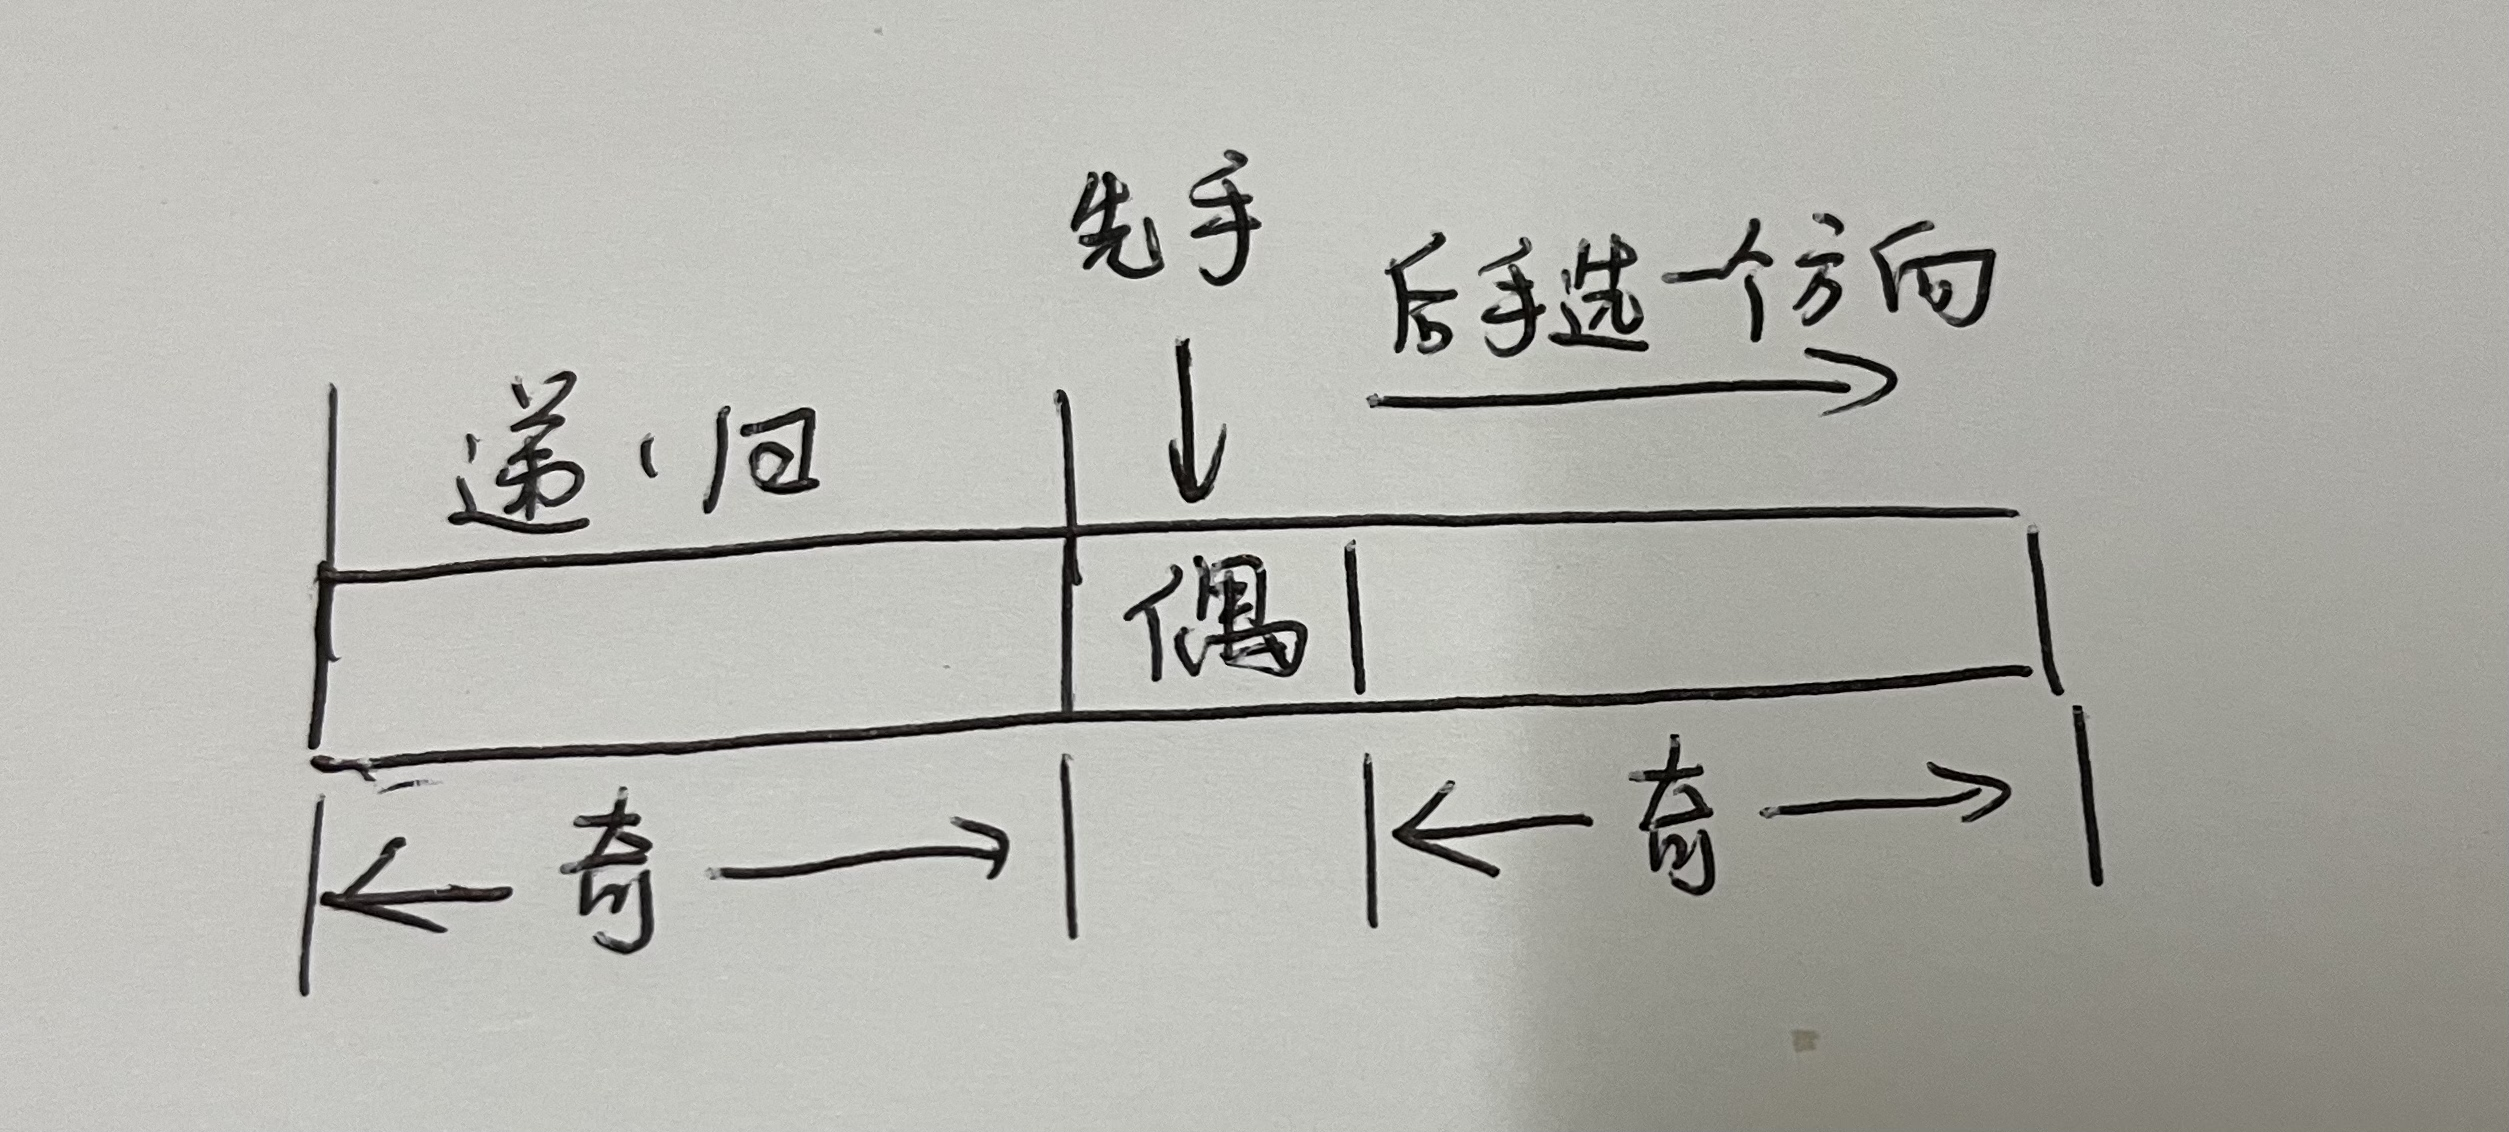
\includegraphics[width=0.5\textwidth]{solutions/img/agc026f/agc026f_1.jpg}
\end{center}

然后考虑取奇数的情况。首先我们发现一点,就是如果开局取奇数,先手得到的是一定不会小于 $A$ 的,因为我们可以 $1, 3, 5, \cdots$ 这样选。然后通过观察我们发现先手得到的也是不可能大于 $A$ 的,因为假设不这样选,先手一开始选了中间的一个 $k$,那么假设后手选择向右取完了 $k\sim n$,取完后我们发现对于 $1\sim k-1$,这一段区间中是原来的后手先选。这时候,后手完全可以 $k-1, k-3, k-5, \cdots$ 来强迫先手达到 $A$。而这只是一种方案,有可能有其他更有方案。因此,$1, 3, 5, \cdots$ 这样取就是最优的。

然后我们摸一下发现是这样的事情:首先先手选了一个偶数,后手选择一段,先手再选一个偶数,后手选择一段……直到某一时刻先手发现自己的最优策略就是把剩下所有的奇数箱子全部取完。这时候先手取完所有剩下的奇数,后手取完剩下的所有偶数,游戏结束。

仔细观察这个过程,我们发现相当于是先手每次选一个偶数点作为“关键点”,这时候后手选择这个关键点向左或向右将某一半的奇数点取走。经过这样的操作。我们发现以这些关键点分段,其实把整个序列分成了很多小的部分,而后手其实是选择了一个部分取走其中的偶数点,而取走其他部分的奇数点。(先手每次选择一个关键点,然后后手朝着离这个想选偶数点的区间的反方向将所有的奇数点取走)。

我们考虑二分答案 $x$,然后先手贪心地将每一段切的都满足这段中的奇数点权和减去偶数点权和小于等于 $x-B$。贪心复杂度 $\mathcal{O}(n)$。

故总复杂度 $\mathcal{O}(n\log\max\{a_i\})$。
\section{POI}

\ptitle{Step Traversing a Tree}{pufanyi}

\prob 给你一棵 $n$ 个点的树,构造一个长度为 $n$ 的 $permutation$,使得 $\forall i, \mathrm{dist}\left\{p_i, p_{i+1}\right\}\le 3$。
\sol $f_u$ 从 $u$ 开始,到 $u$ 的一个叶子节点结束,遍历以 $u$ 为根子的答案树;$g_u$ 表示从 $u$ 的一个叶子节点开始,到 $u$ 结束遍历以 $u$ 为根子树的答案。发现两者可以相互递归调用。
\section{ICPC}

\ptitle{[2023 Macau A] 	(-1,1)-Sumplete}{shaosy}
\prob 给定一个$n\times n$的矩阵, 每个元素是$1$或者$-1$, 要求选定一些元素置零, 使得每一行的和为$r_i$, 每一列的和为$c_i$
\sol 将所有$-1$看作$0$, 然后操作就变成选定一些点$i,j$, 对第$i$行和第$j$列的和减1. 这一问题可以贪心求解 (每一行选择剩余可以减去的最多的列减去即可).

\ptitle{[2023 Macau E] 	Inverse Topological Sort }{shaosy}
\prob 给定一张图的字典序最小/最大的拓扑序, 要求复原这张图
\sol 考虑字典序最小的拓扑序$a$. 若$i < j$且$a_i > a_j$, 则若$a_i$和$a_j$联通, 则点$a_i$和$a_j$之间要么直接连边, 要么必然存在间接边使得$a_i$能指向$a_j$. 这样可以构造一组$n^2$条边的图满足题意. 可以仅考虑最大的$i$满足$a_i > a_j$与$a_j$相连. 这一组仍然满足原有的偏序关系. 对字典序最大的拓扑序同理. 建图后check即可.